\documentclass[tikz,border=5pt]{standalone}
\usepackage{luatexja}
\usepackage[hiragino-pron]{luatexja-preset}
\usepackage{amsmath,amssymb}
\usetikzlibrary{arrows.meta}

\begin{document}
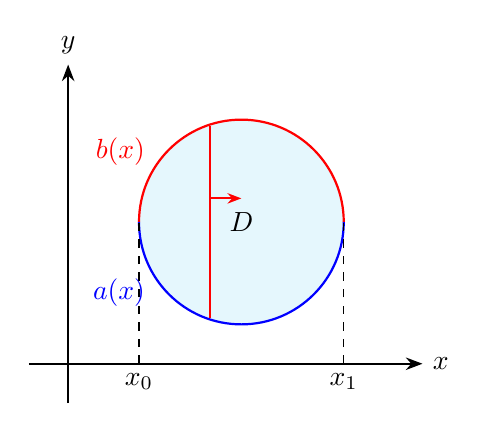
\begin{tikzpicture}

% Parameters
\def\cx{2.2}   % circle center x
\def\cy{1.8}   % circle center y
\def\cr{1.3}   % circle radius

% Axes
\draw[-{Stealth[length=6pt]}, thick] (-0.5,0) -- (4.5,0) node[right] {$x$};
\draw[-{Stealth[length=6pt]}, thick] (0,-0.5) -- (0,3.8) node[above] {$y$};

% Fill region D
\fill[cyan, opacity=0.1] (\cx,\cy) circle (\cr);

% Circle: upper half red, lower half blue
\draw[red, thick] (\cx,\cy) ++(0:\cr) arc[start angle=0, end angle=180, radius=\cr];
\draw[blue, thick] (\cx,\cy) ++(180:\cr) arc[start angle=180, end angle=360, radius=\cr];

% D label
\node at (\cx,\cy) {$D$};

% Vertical red arrow inside D at x = 1.8 (inner integral direction: a(x) → b(x))
% Circle at x=1.8: y = cy ± sqrt(cr^2 - (1.8-cx)^2) = 1.8 ± 1.237
\def\ax{1.8}
\pgfmathsetmacro{\adx}{\ax-\cx}
\pgfmathsetmacro{\ady}{sqrt(\cr*\cr - \adx*\adx)}
\draw[red, thick]
  (\ax,{\cy-\ady+0.02}) -- (\ax,{\cy+\ady-0.02});
% Right-pointing arrow from middle of red line
\draw[-{Stealth[length=5pt]}, red, thick]
  (\ax,{\cy+0.3}) -- ++(0.4,0);

% Dashed lines from circle to x-axis (x0, x1)
\draw[dashed, thin] ({\cx-\cr},0) -- ({\cx-\cr},{\cy});
\draw[dashed, thin] ({\cx+\cr},0) -- ({\cx+\cr},{\cy});


% Labels
\node[below] at ({\cx-\cr},0) {$x_0$};
\node[below] at ({\cx+\cr},0) {$x_1$};
\node[above left, red] at ({\cx-1.1},{\cy+0.6}) {$b(x)$};
\node[below left, blue] at ({\cx-1.1},{\cy-0.6}) {$a(x)$};

\end{tikzpicture}
\end{document}
